	\chapter{Materials and Methods}
\label{cha:MaterialsAndMethods}

	\section{Databases}
	\label{sec:Databases}
	In the present study various databases have been used to retrieve sequence (DNA and Protein) and protein structure information. For the sequence analysis in Section \ref{sec: ACPSequenceAnalysis} RefSeq microbial and UniProtKB/TrEMBL (with 6408654 seq and 20127441 seq respectively, as on 9$^{th}$ March, 2012) were used to search for ACP homologues using the hidden Markov models. RefSeq is a non-redundant database of DNA, RNA and protein sequences curated by the sequences from International Nucleotide Sequence Database Collaboration (INSDC) hosted at the National Centre for Biotechnology Information (NCBI) \nomenclature{NCBI}{National Centre for Biotechnology Information}. RefSeq (\url{http://www.ncbi.nlm.nih.gov/refseq/}) provides the reference sequence for a species, each entry being annotated and cross-linked to other databases by collaborating groups and NCBI staff. RefSeq can be accessed via the Entrez search engine, through a sequence similarity search using BLAST \nomenclature{BLAST}{Basic Local Alignment Search Tool} or by the RefSeq FTP server. The RefSeq microbial dataset was used, which consists of sequences from microbial genomes/proteomes. 

	UniProtKB/TrEMBL (\url{http://www.uniprot.org}) is a collection of computationally annotated protein sequences. The sequences in UniProtKB/TrEMBL are derived from the computational translation of the coding sequences (CDS) submitted in INSDC databases. UniProtKB/TrEMBL can be accessed through keyword or uniprot identifier searches on the UniProtKB website or through a sequence similarity search using BLAST. The purpose of selecting two databases was not only to retrieve the highest quality sequence information from a curated database but also to have maximum coverage of sequences available through an automated database. The sequence data from both the databases were obtained from their FTP websites in the FASTA format.
	
	For molecular modelling, as explained in Section \ref{sec:HomologyModelling}, protein structure coordinate information was taken from the Protein Data Bank (PDB) \nomenclature{PDB}{Protein Data Bank} (\url{http://www.rcsb.org}). The PDB is the single archive for macromolecule (DNA and Protein) 3D coordinate information. It consists of structural information determined through experimental methods such as NMR spectroscopy and X-ray crystallography. The PDB database can be searched by keyword or PDB identifier, or by running a BLAST similarity search either from within the PDB website or through NCBI BLAST.
	
	\section{Sequence analysis}
	\label{sec:SequenceAnalysis}
	In molecular biology, routine sequence analysis is carried out to infer the biological function of newly sequenced DNA or protein sequences. For the purpose of inferring biological function similarity searches against annotated sequence databases using pairwise alignment methods such as BLAST and FASTA are in common use. Pairwise sequence alignment methods give equal weighting to all aligned positions. However, in a multiple sequence alignment it can be clearly seen that several positions within a family of proteins are under more evolutionary pressure to be conserved than others. Thus pairwise sequence alignment methods are good for fast searches of closely related sequences but are poor at detecting remote homology. In contrast, methods based on position specific scoring and probability such as Profiles and hidden Markov models are much more sensitive in detecting remote homology. 
		
		\subsection{PSI-BLAST and multiple sequence alignment}
		\label{sec:PSIBlastAndMSA}
		In the present study position specific iterative BLAST (PSI-BLAST) has been used to identify template structures for homology modelling (see Section \ref{sec:HomologyModelling}). PSI-BLAST is an extension of the normal protein-protein BLAST but it uses a position specific scoring matrix (PSSM) or profile. This PSSM is generated from the multiple sequence alignment of the sequences found in a normal protein BLAST, which is the first iteration of PSI-BLAST. The PSSM is used and refined in further iterations of PSI-BLAST, rather than a simple sequence. PSI-BLAST is more sensitive in detecting distantly related sequences as compared to the normal protein-protein BLAST. 
		
		In Section \ref{sec: ACPSequenceAnalysis} multiple sequence alignments (MSAs) were used to identify conserved residues which differentiate branching-ACPs from non-branching-ACPs. An MSA is created with three or more sequences with the aim of identifying regions of sequence homology and conserved positions, which may be used to characterize a protein family. MSAs are also used for phylogenetic reconstructions as differences between sequences, can be used to estimate how recently two proteins from a given family a common ancestor in a family of protein/DNA sequences. As explained in Section \ref{sec:ET} MSAs were also used for evolutionary trace analysis to predict positions under evolutionary pressure within a clade as compared to between the clades. The ClustalW and Muscle programs were used for generating MSAs.
		
		\subsection{Hidden Markov models (HMMs)}
		\label{sec:HMM}
		HMMs are models which represent a probability distribution of the occurrence of residues for each position in a multiple sequence alignment allowing for the residue type to occur through conservation, insertion, deletion, or some combination of the later two with the aim of encapsulating the common features of a protein family that are necessary to recognize other members of the family. HMMs are built on a set of aligned sequences belonging to a family of proteins. Each column in an MSA is considered as a \textquotedblleft state\textquotedblright which \textquotedblleft emits\textquotedblright symbols (residues) according to the emission probabilities. Each state is interconnected to other states called transitions with state transition probabilities. The model produces the sequence of symbols based on the emission and transition probabilities and the probability of a given sequence being produced is the product of all the emission and transition probabilities. The hidden part in a hidden Markov model is the sequence of the states taken to produce the sequence of symbols. It’s only the “emitted” symbols which are visible, not the underlying state. In practice HMMs are generated (or trained) using an MSA. To align a sequence to an HMM model the HMM can be seen as traversing all the possible sequences of states through the model to generate the target sequence. This will assign the probability values to the sequences produced of which the best ones are selected through a dynamic programming based algorithm such as the Viterbi algorithm.
		
		\subsubsection{HMM analysis of \bet-branching and standard ACPs}
		\label{sec:HMMACPs}
		HMMs were used to classify a subclass of acyl carrier proteins (ACPs) called the branching ACPs (for results see Section \ref{sec: ACPSequenceAnalysis}). The two HMM models were built using the HMMER program from the 15 clusters with known pathways, with 38 and 178 sequences (sequences provided by Dr. Anthony Haines) for the branching and the non-branching-ACPs respectively. The training and the test set were scored with each HMM models and the scores were plotted on a scatter graph to highlight two distinct clusters between branching and non-branching ACPs. The non-branching HMM model was also searched against TrEMBL and RefSeq databases which fetched 16,490 unique sequences with the length greater or equal to 60 amino acids. These sequences were also scored with both the models and plotted in a separate scatter plot along with the training set.  The models were deposited with SMART since no domain prediction software (SMART, Pfam etc.) had the capacity to distinguish these two types of ACP.
	
	\section{Molecular Modelling}
	\label{sec:MolecularModelling}
	The present study aims to model the polyketide synthase complexes which are large macromolecular complexes. Determining the structure of large protein complexes through experimental methods such as X-ray crystallography and NMR \nomenclature{NMR}{Nuclear Magnateic Resonance} spectroscopy is possible however at times can be quite difficult and time consuming. On the other hand with the increase in computing capacity and the large amount of molecular biology data available it is increasingly possible and efficient to use computational methods to predict structures based on the existing structural data. Molecular modelling can be used for tasks such as protein structure prediction through homology modelling, understanding protein dynamics through molecular dynamics simulations, protein – protein interaction interface prediction and molecular docking to generate atomic resolution three dimensional protein complex structures. 
	
		\subsection{Homology modelling}
		\label{sec:HomologyModelling}
		Homology modelling or comparative modelling is a computational method to generate three dimensional protein structures of atomic resolution. As the name suggests homology modelling is based on the fact that the proteins which perform similar functions tend to have similar sequences with regions important for the function being conserved. Furthermore, the protein structures of even divergent protein sequences, which share a common ancestry, tend to fold into a similar three-dimensional structure. Thus a protein structure can be used to predict the atomic resolution model of a homologous target sequence \Parencite{Chothial1986}. The theoretical models generated through homology modelling primarily rely on the quality of the sequence alignment between the target sequence and the homologous sequence and the quality of the homologous structure. Over the past few years several state of art computational tools have emerged with increasing level of accuracy, which are continually being monitored by the biannual CASP competitions (\url{http://predictioncenter.org/}).
		
		In the present work, different versions of the Modeller \Parencite{Sali1993} program have been used to carry out the homology modelling for all the predicted structures. Modeller generates the three dimensional models of the target protein sequence by satisfying spatial restraints obtained from the sequence alignment of the target and the homologous protein templates. This method in principle is quite similar to employing the distance geometry approach used in NMR experiments. The spatial restraints extracted from the sequence alignment are expressed as probability density functions (PDFs) which are used to restrain C$\alpha$-C$\alpha$ bond distance, N-O distance, main chain and side chain dihedral angles. Apart from the bond distance restraints derived from the sequence-template alignment, stereochemical restraints are added using a molecular mechanics force field. In the final model building step the model is generated by minimizing the violation of all the restraints \Parencite{Marti-Renom2000, Eswar2006}.
		
		This method of model prediction has an advantage over many other tools for the same purpose as it allows several restraints to be added by the user derived from various resources. It is thus possible to apply restraints derived from experiments such as NMR spectroscopy, fluorescence resonance energy transfer (FRET), crosslinking experiments as well as restraints derived from Bioinformatics based experiments. The model building step can also be coupled with model refinement steps using simulated annealing and molecular dynamics simulations. However, in the present work many of the models were generated without any model refinement step which allows a direct comparison with the template structure as the algorithm places the side chains at the similar positions to the template. %Here Modeller has also been used to model homodimeric proteins for example the ketosynthase homo dimer in MmpA, as found in the X-ray structure of the ketosynthase - acyltransferase didomain of module 5 from DEBS systems (PDB ID 2HG4).
		
			\subsubsection{Modelling of MupH + ligand complex}
			\label{sec:HomologyModellingMupH}
			MupH was modelled using Modeller version 9.8 \Parencite{Eswar2006}. The MupH sequence was used to search the PDB for the solved homologous structures, using PSI-BLAST. 10 structures were selected ranging from 27\% to 32\% sequence identity to generate the initial alignment using ClustalW \Parencite{Larkin2007}. The structures chosen in similarity with the MupH sequence were from the species \textit{Staphylococcus auereus, Enterococcus faecalis, Brassica juncea, Streptococcus mutans} and \textit{Homo sapiens} thus providing a wide range of organisms for comparisons. All the homologues found were HMG-CoA synthases. The secondary structures of the templates, determined by DSSP \Parencite{Joosten2011}, guided manual refinement of the final alignment using Seaview \Parencite{Galtier1996}. The HMG-CoA synthase structure from \textit{Enterococcus faecalis} (PDB ID 1X9E), having 87\% query coverage with 32\% sequence identity, was selected as the template. Modeller produced five structures which were further tested for stereochemical quality using the PROCHECK \Parencite{Laskowski1993} program (\url{http://nihserver.mbi.ucla.edu/SAVES/}). The model with the best PROCHECK score was selected for further analysis. 
			
			In order to dock the polyketide intermediate ligand in the MupH active site the modelled MupH structure was superimposed on the 1X9E crystal structure and the X-ray determined coordinates for the phosphopantetheine moiety from the bound ligand in 1X9E were copied. The rest of the polyketide intermediate was built manually inside the MupH active site using the PyMol program (\url{http://www.pymol.org}). To remove the steric clashes energy minimization was carried out using Chimera \Parencite{Pettersen2004}. The AMBER99SB-ILDN \Parencite{Hornak2006} force field and Antechamber program were used to assign the force field parameters to the protein and ligand respectively. 
			
			\subsubsection{Modelling of ACP-mupA2}
			\label{sec:ACP2modelling}
			ACP-mupA2 (the ACP from the second module of MmpA in the mupirocin cluster) was modelled using Modeller version 9.10. The ACP-mupA2 sequence (GenPept Acc No. AAM12909 range 1822 to 1916) was used to search against the PDB database using BLAST to identify the template. The NMR structure of the Holo-Acpi Domain from the CurA module from \textit{Lyngbya Majuscula} (PDB ID 2LIU) was selected as the best template with 80\% query coverage and 29\% sequence identity. To generate the initial alignment for modelling, a multiple sequence alignment was carried out using two template sequences, 2LIU, 2L22 (ACP-mupA3ab NMR structure from the third module of MmpA in the mupirocin cluster) and other ACP sequences from the mupirocin cluster. Sequence alignment was manually refined using secondary structure information as explained in Section \ref{sec:HomologyModellingMupH} and the homology modelling was carried out using 2LIU as the template, generating five structures. The structures were tested for stereochemical quality using PROCHECK and the structure with the best PROCHECK score was selected for further analysis. 
			
			\subsubsection{Modelling of the KS-mupA2 dimer}
			\label{sec:KS2modelling}
			KS-mupA2 (KS from the second module of MmpA in the mupirocin cluster) was modelled using Modeller version 9.11. KS-mupA2 was modelled as a dimer along with the KS docking domain also called as the linker region between the KS and AT domain in the \textit{cis} systems. KS-mupA2 sequences (GenPept Acc No. AAM12909.2 range 715 to 715 to 1288) was searched against the PDB database using BLAST to identify the template. Two templates from the DEBS system, the KS-AT dimer from module three and five (PDB ID 2QO3 and 2HG4) along with the KS sequences from the mupirocin system, were used to generate the initial alignment which was manually refined using secondary structure information and visual inspection of the alignment. The DEBS structure 2QO3 with 88\% query coverage and 39\% sequence identity was used as the template to generate five homology models. The structures were tested for stereochemical quality using PROCHECK and the structure with the best PROCHECK score was selected for further analysis.
		
		\subsection{Molecular dynamic simulation}
		\label{sec:MolecularDynamicSimulation}
		Molecular dynamic (MD) simulation is a computational method to simulate the time dependent behaviour of a physical system. In molecular modelling, MD simulations of proteins and DNA macromolecules are used to observe the changes in forces and structural dynamics with respect to time. In a typical MD simulation of a physical system of N interacting atoms, such as a protein immersed in a box of solvent, the atoms are allowed to move following Newton's laws of motion. Equation \ref{eq:force} represents the differential form of Newton's second law of motion i.e. F=ma, describing the motion of a particle \textit{i} of mass $ m_{i} $, in the direction $ x_{i} $ with the force $ F_{x_i} $ acting on the particle in the $ x_{i} $ direction. %force F$ _{i} $, on a particle i with coordinates r$ _{i} $, which is equal to the product of mass of the particle m$ _{i} $  and its acceleration. 
		
		\begin{equation}
		\label{eq:force}
			\frac{\delta^2x_i}{\delta t^2} =  \frac{F_{x_i}}{m_i}, i=1 ... N
		\end{equation}
		
%		\noindent Where force is the negative derivative of the potential function $V (r_1, r_2 ... r_N)$.
%		
%		\begin{equation}
%		\label{eq:force1}
%			F_i = - \frac{\delta V}{\delta r_i}
%		\end{equation}
		
		\noindent The calculation of the forces highly depends on the parameters of the molecular mechanics force field equation used. The equation below is the functional form of the AMBER force field equation.
		
		\begin{equation}
		\label{eq:AMBER}
		\begin{gathered}
			V(r^N) = \sum k_b (l-l_0)^2 + \sum k_a (\theta - \theta_0)^2 + \sum \frac{1}{2} V_n [1 + \cos(nw - \gamma)] \\ 
			+ \sum_{j=1}^{N-1} \sum_{i=j+1}^{N} \Biggl \lbrace \Biggl[\epsilon_{ij} \left(  \frac{r_{0ij}}{r_{ij}} \right)^{12} - 2 \left(\frac{r_{0ij}}{r_{ij}}\right)^6 \Biggl] + \frac{q_i q_j}{4 \pi \epsilon_0 r_{ij}} \Biggl\rbrace
		\end{gathered}			
		\end{equation}
		
		The first term in the equation represents the energy of the covalent bonds. The second term represents the energy of the bond angles. The third term represents the energy due to torsional angles and the last term represents the energy due to non-bonded interaction between all the atom pairs, which include van der Waals, and electrostatic energies. 
		
		In molecular dynamics simulation the equation of Newton's second law of motion is solved for the desired length of time. %at the required temperature and pressure. 
		The change in the coordinates of the atoms due to the motion is recorded at regular intervals. The coordinates with respect to time represents the trajectory of the system. Once the system has reached the equilibrium state many macroscopic properties can be studied by averaging over the equilibrium trajectory. MD simulations are widely used in molecular modelling to study folding and unfolding of the proteins, protein structure stability, protein-protein interactions, free energy binding of drug-protein complexes, the effects of mutations on the structural dynamics of the proteins etc. 
		
		In the present study the GROMACS 4 \parencite{Pronk2013} molecular dynamics program has been used to study the protein dynamics in explicit solvent (water) and the protocol can be summarized in three major steps. 
		
		\begin{description}
		\item[Structure preparation] \hfill \\ In the first step, the physical system to be simulated is represented in the computer. The protein structure from X-ray or NMR experiments or through homology modelling contains the coordinate information only. However, for running the MD simulation this coordinate information needs to be expressed in terms of atomic coordinates, atom types, bonds, electric charge distribution etc. This information is stored in a topology file along with the necessary force field parameters from the selected force field and the water model to be used for the explicit solvent simulation. There are several popular force fields supported by GROMACS, which includes GROMOS \parencite{Oostenbrink2004}, AMBER \parencite{Lindorff-Larsen2010}, OPLSA \parencite{Jorgensen1996}, and the CHARMM27 \parencite{MacKerell1998} force fields. During the structure preparation step hydrogen atoms (if any are present) are usually removed from the coordinate file and added back according to the specifications of the force field used. This rebuilding of hydrogen atoms may cause some steric clashes which need to be relaxed through energy minimization. 
		
		For simulations in explicit solvent usually a simulation box is created with periodic boundary conditions (PBC) which is filled with a suitable water model for example SPC, TIP3P \parencite{Spoel1998}. There are a few limited number of shapes in which the simulation box can be created with a cube being the largest in terms of the volume and truncated dodecahedron being the smallest. A truncated dodecahedron surrounds spherical globular proteins better because it does not accumulate huge amount of solvent at the corners therefore it is computationally less expensive than e.g. a cube. The PBC means a single unit is repeated infinitely in order to overcome the edge effects caused by the walls of the simulation box. %Once the box is setup it is filled with the water molecules chosen in the first step. There are several water models available with preference for different force field equations. 
		For the Amber force field used in the present work the TIP3P water model is considered a compatible model and was used here. At this point once the solvation box is created and filled with the suitable solvent the net charge of the system is neutralized by adding counter ions. The energy of the system is minimized either using a steepest descent algorithm, conjugate gradient algorithm or both to remove any steric clashes \parencite{Hess2008a}.
					
		\item[Equilibration and production run] \hfill \\  In the second step, the system is equilibrated by running short MD simulations in which the protein is restrained to the reference position while keeping the water molecules flexible. This allows the water molecule to relax around the protein. %as well as reach the system to the desired temperature and pressure. 
		It is a general practice to first run a short simulation with only temperature coupling to equilibrate the system at the desired temperature for example at 300K. Once the system is equilibrated at the desired temperature another short simulation can be run with the pressure coupling as well to equilibrate the system under both the temperature and pressure conditions. These equilibration steps are usually performed for few hundred pico seconds depending upon the size of the system. 
		
		In the final production run, MD simulation is carried out without any restrains on the protein under the influence of temperature and pressure, which can be of several nanoseconds long depending upon the macroscopic property under study and the computational power available \parencite{Hess2008a}. 
		\end{description}
		
			\subsubsection{Parameter determination}
			\label{sec:MDparameters}
			As mentioned above, the forces in the simulation depend on the parameters used. These parameters include atomic properties such as mass, partial charge and atom type, bond properties such as equilibrium bond length, equilibrium bond angle and dihedral angle preferences and parameters representing the partial charges  and van der Waals interaction. Since, forcefields in GROMACS are optimized for protein and nucleic acid simulation, parameters are given only for the standard amino acids, nucleotides and a few counter ions. However, GROMACS allows the addition of extra parameters to represent systems which consist of atoms not represented by the standard set of parameters. In order to include a molecule which is not a part of the standard set, different methods based on either experimental data or quantum mechanics calculations can be used to determine parameters. While working with the AMBER force fields small molecules can be simulated using parameters from the general amber force field (GAFF). GAFF was created to be compatible with the AMBER force fields \parencite{Wang2004} and is part of the AMBER molecular dynamics package which is not included in GROMACS by default. 
			
			In the present study at several instances a ligand molecule was covalently attached to a residue in the protein, for example a phosphopantetheine arm attached to the active site serine in an ACP. To carry out molecular dynamics simulation with the phosphopantetheine and other molecules attached to the serine on ACP a new residue type was created for each serine ligated with ligand. Since, these new residues were not a part of the standard amino acid set, GROMACS did not have the parameters to carry out the simulation. For this reason parameters from the GAFF were added to the AMBER 99SB-ILDN \parencite{Lindorff-Larsen2010} force field. The GAFF parameters were obtained from the AMBER molecular dynamics package and the values which differed in units from GROMACS format where converted using several in house perl scripts (see Appendix I \ref{sec:gafftogro}).
			
			While using GAFF in AMBER molecular dynamics package, partial atomic charges (AM1-BCC) are assigned using antechamber software included in the package. However, in GROMACS suite there was no such software available which can assign partial atomic charges to small molecule. %Every force field supported by GROMACS have charges for standard amino acids, nucleotides and few metal ions in their corresponding databases. 
			Therefore, in order to derive partial atomic charges for the new residues, AMBER force field compatible RESP charges were calculated using RED server (\url{http://q4md-forcefieldtools.org/REDS/} \parencite{Bayly1993, Dupradeau2010b, Vanquelef2011}). For the calculation of RESP charges the RED server requires the structure file in a P2N format. The program Ante RED, available in the RED server, converts a  PDB file into the P2N format. The RED IV server was used to calculate RESP-A1A charges for all the ligands, using the Gaussian 2009 D.01 quantum mechanics program. Fully automated mode 1 was chosen while running RED IV which performs geometry optimisation as well as charge fitting. Once the charges were calculated a new entry was created for each new residue type in the \textit{aminoacids.rtp} database of GROMACS. The new residue name was also updated in the \textit{residuetype.dat}  database. For each new residue the corresponding hydrogen atoms were also created in the \textit{aminoacids.hdb} database. While determining charges for the new moiety attached to an existing amino acid, the charges for the serine side chain were varied but the backbone atoms of the parent residue were kept the same as that of the original forcefield. Section \ref{sec:newresidues} in Appendix II lists the ligands with the charges which were added to the AMBER99SB-ILDN \textit{aminoacids.rpt} database.
				
			\subsubsection{Molecular dynamics simulation of W44L mutant and wild type ACP-mupA3a}
			\label{sec:WtoL_MD}
			A) The mutation from W to L at the $44^{th}$ position in the ACP-mupA3a NMR structure was carried out using PyMol. The two constructs (wild type and the mutant) were subjected to 20 independent simulations for 10 ns each. The GROMACS 4 \parencite{Hess2008a} molecular dynamics engine with AMBER99SB-ILDN \parencite{Lindorff-Larsen2010} force field and TIP3P water model was used to carry out the simulation with a time step of 2fs and in a water box extending 5 {\AA }  beyond the surface of the protein. The simulation systems were each neutralized with 2 Na$ ^{+} $ counter ions, minimized for 1000 steps of conjugate gradient and 1000 steps of steepest descent energy minimisation and were equilibrated for 100 ps. The final simulation run was performed for 10 ns at 300K temperature and 1 atm pressure with other parameters set as the GROMACS 4 defaults.
			
			B) Another set of two independent simulations were setup for the W44L mutant and wild type ACP-mupA3a for 1 microsecond each. The simulation systems were neutralized by adding 2 Na$ ^{+} $ counter ions and the protocol and the setup was same as described in Section \ref{sec:SPTsimulation}.
			
			\subsubsection{Molecular dynamics simulation of ACP-mupA3a with covalently bound phosphopantetheine}
			\label{sec:SPTsimulation}
			The ACP-mupA3a NMR structure was simulated with the phosphopantetheine covalently attached to S38 of both the wild type ACP-mupA3a and W44L ACP-mupA3a mutant. In order to simulate phosphopantetheine covalently attached to S38 a new residue named SPT was introduced in the GROMACS \textit{aminoacids.rtp} database (Appendix II Section \ref{sec:SPTcharge}). The structure for SPT was drawn using Pymol by extending S38 coordinates from the NMR structure (PDB ID 2L22). Parameters for the serine backbone atoms were kept the same as that of the original AMBER99SB-ILDN forcefield and for the rest of the ligand (from phosphate onwards) were derived from GAFF. Charges for the phosphopantetheine moiety were determined  using  the RED server as described in Section \ref{sec:MDparameters}. The structure file used for charge calculation consisted of a phosphopantetheine moiety attached to the serine side chain oxygen with all the atoms of the serine present and the backbone carbonyl carbon and amide nitrogen blocked with methyl groups. After charge fitting with RED server, the charges on the serine backbone were set to the same values ass the AMBER99SB-ILDN force field, the blocking methyl groups were removed, and the remaining charges were adjusted in the third decimal places to keep the overall charge of the molecule as -1 %While keeping the charges for the serine backbone atoms the same as that of the AMBER99SB-ILDN forcefield, the difference in the charges upon removing the  methyl groups used for blocking, were adjusted in other atoms to keep the overall charge of the molecule as -1 
			(Appendix II Section \ref{sec:SPTcharge}).
			
			The two constructs (wild type and the mutant) were subjected to 5 independent simulations for 50 ns each. Simulations were carried out using TIP3P water with a time step of 2fs and placed in an octahedron water box extending 10 {\AA }  beyond the surface of the protein. Each simulation system was neutralized with 3 Na$ ^{+} $ counter ions and minimized for 1000 steps of conjugate gradient and 1000 steps of steepest descent energy minimisation. Following the energy minimisation each system was equilibrated with 100 ps of NVT and 100 ps of NPT simulations keeping the position of the protein atoms restrained. The final simulation was performed for 50 ns at 300K temperature and 1 atm pressure using V-rescale thermostat \parencite{Berendsen1984} and Parrinello-Rahman pressure coupling \parencite{Parrinello1980} respectively. Out of the five simulations per construct one was extended for to 200 ns for both wild type and mutant ACP-mupA3a.
			
					
			\subsubsection{Molecular dynamics simulation of ACP-mupA3a with its substrate}
			\label{sec:SPMsimulation}			
			ACP-mupA3a wild type and W44L ACP-mupA3a mutant were simulated with their substrate prior to \bet-branching (Figure \ref{fig:muppathway}). The ACP-mupA3a substrate was built directly onto the phosphopantetheine  of Section \ref{sec:SPTsimulation} by using PyMol. All the bond parameters and charges for the phosphopantetheine moiety were kept the same as the previous calculations. Parameters for the ACP-mupA3a substrate were obtained from GAFF and charges were calculated using the RED server. The charge calculations were performed on the ACP-mupA3a substrate attached to a sulphur and peptide moiety, representing the terminal atoms of the phosphopantetheine arm, the peptide being blocked by the addition of a methyl group. Including the entire phosphopantetheine in charge calculations was not preferred as it showed to bias the geometry optimization in a U shaped conformation rather than an extended one and these interactions would polarize the charges. HG-63G* charges already over polarize the charges compared to gas phase, to mimic the effect of intermolecular interactions \parencite{Winn1997} Therefore, the charges were calculated separately and then merged with the previously calculated charges for the phosphopantetheine, keeping the overall charge on the molecule as -1. The new residue, SPM, was added into the AMBER99SB-ILDN \textit{amoniacids.rtp} database in GROMACS (Appendix II Section \ref{sec:SPMcharge}). The simulation system was neutralized by adding 3 Na$ ^{+} $ counter ions and five independent simulations were carried out for 50 ns each following the same protocol as described in Section  \ref{sec:SPTsimulation}. One of the simulations was extended to 1 $ \mu $s for the wild type ACP-mupA3a and upto 200 ns for the W44L ACP-mupA3a mutant. 

			\subsubsection{Molecular dynamics simulation of ACP-mupA3a with a covalently bound saturated carbon chain}
			\label{sec:SPCsimulation}
			ACP-mupA3a wild type was simulated with a covalently bound 14C saturated chain to the phosphopantetheine. The carbon chain was of the same length as that of the ACP-mupA3a substrate's backbone. The parameters and the charges for the phosphopantetheine moiety were the same as in the previous calculations. The parameters for the 14C saturated carbon chain was obtained from GAFF and the charges were calculated using RED server. The new residue SPD was added into the AMBER99SB-ILDN \textit{amoniacids.rtp} database in GROMACS (Appendix II Section \ref{sec:SPCcharge}). The simulation system was neutralized by adding 3 Na$ ^{+} $ counter ions and three independent simulations were carried out for 50 ns each following the same protocol as described in Section  \ref{sec:SPTsimulation}. One of the simulations was extended upto 200 ns. 
			
			\subsubsection{Molecular dynamics simulation of ACP-mupA2a with its substrate}
			\label{sec:SPBsimulation}
			ACP-mupA2a wild type was simulated with its substrate (Figure \ref{fig:muppathway}). All the parameters for the phosphopantetheine moiety were the same as in the previous calculations. Parameters for the ACP-mupA2 substrate were obtained from GAFF with charges calculated using the RED server. The new residue SPB was added into the AMBER99SB-ILDN \textit{amoniacids.rtp} database in GROMACS (Appendix II Section \ref{sec:SPBcharge}). The molecular dynamics simulation procedure was as in the Section \ref{sec:SPTsimulation}. The simulation system was neutralized by adding 5 Na$ ^{+} $ counter ions and three independent simulations were carried out for 50 ns each following the same protocol as described in Section  \ref{sec:SPTsimulation}. One of the simulations was extended to 200 ns. 
			
			\subsubsection{Molecular dynamics simulations of ACP-mupA3a:MupH complex}
			\label{sec:mdAcpMuph}
			The starting configuration for MD simulation of the ACP-mupA3a:MupH complex was a representative complex from the \textit{in silico} docking described in Section \ref{sec:acpMuphDocking} and Chapter \ref{cha:ACP-HCS} Section \ref{sec:MupHACPInteraction}. ACP-mupA3a had its substrate attached to the phosphopantetheine. %The conformation of the phosphopantetheine and the monic acid was made as close to the previous docking conformation as possible by aligning the two ligands together. 
			An acetyl molecule was covalently attached to the C115 in the MupH active site. The force field parameters for the phosphopantetheine and ACP-mupA3a substrate were taken from the previous calculations as described in section \ref{sec:SPMsimulation}. Parameters for the acetyl molecule attached to the C115 were obtained from GAFF with the charges calculated by using the RED server. A new residue type CYA for C115Acetylated-cysteine was introduced into the AMBER99SB-ILDN \textit{amoniacids.rtp} database in GROMACS (Appendix II \ref{sec:CYAcharge}). The simulation system was neutralized by adding 16 Na$ ^{+} $ counter ions and three independent simulations were carried out for 50 ns each following the same protocol as described in Section  \ref{sec:SPTsimulation}. One of the simulations was extended upto 100 ns.
			
			Another set of simulations were carried out for ACP-mupA3a:MupH complex but with MupH as a dimer. All the parameters were kept the same as that for the ACP-mupA3a:MupH monomer complex. However, new topologies were generated including the MupH dimer. The ACP-mupA3a:MupH dimer system was neutralize by adding 29 Na$ ^{+} $ counter ions. Three independent simulations were carried out for 50 ns each following the same protocol as described in Section  \ref{sec:SPTsimulation}.
			
			\subsubsection{Molecular dynamics simulations of MupH and MupH acetylated at C115 in isolation}
			\label{sec:muphCya}
			Three independent simulations for MupH and MupH acetylated at C115 were carried out for 50 ns each. The force field parameters for the acetyl molecule attached to the C115 were from previous calculations (as described in Section \ref{sec:mdAcpMuph}). The simulation systems for both the structures were neutralized with 13 Na$ ^{+} $ counter ions and were carried out following the same protocol as described in Section  \ref{sec:SPTsimulation}.
			
			\subsubsection{Calculating the RMSD and RMSF of ACP-mupA3a and ACP-mupA2 from their reference starting structure}
			\label{sec:RMSDstartingStructure}
			Root mean square deviations (RMSD) of the backbone atoms from the reference starting structure were calculated for all the extended simulations of ACP-mupA3a and ACP-mupA2 using the GROMACS module \textit{g\textunderscore rms}. Below is an example command to run \textit{g\textunderscore rms}, which requires a MD simulation input file and a MD simulation output trajectory file. The RMSD was calculated at every 10 ps of the simulation. The RMSD plots were visualized using the program Grace (\url{http://plasma-gate.weizmann.ac.il/Grace/}). 
			
\begin{lstlisting}
g_rms -s md.tpr -f md.xtc -o rmsd.xvg
\end{lstlisting}			
			
			Root mean square fluctuations (RMSF) were calculated for the backbone atoms, averaged per residue, for all the extended simulations of ACP-mupA3a and ACP-mupA2 using the GROMACS module  \textit{g\textunderscore rmsf}. Below is an example command to run \textit{g\textunderscore rmsf}, which requires a MD simulation input file and a MD simulation output trajectory file. The RMSF was calculated from points in the trajectory at 10 ps intervals. A combined scatter graph was plotted for all the simulations using a spread sheet program. 

\begin{lstlisting}
g_rmsf -s md.tpr -f md.xtc -o rmsf.xvg -res
\end{lstlisting}			
			
			
			\subsubsection{Calculating RMSD of the ACP-mupA3a and ACP-mupA2 from the reference FAS ACP structure}
			\label{sec:RMSDFASACP}
			The GROMACS suite has a module to calculate RMSD of a set of atoms from a reference structure, but it does not perform well with a reference structure which is not identical to the structure in the simulation. The task in this analysis was to calculate the RMSD of the conformational states of the ACP-mupA3a and ACP-mupA2 (wild and mutant) structures at every ns of the simulation from the reference FAS ACP structure (PDB ID 1L0I). To perform this task not natively supported by GROMACS, conformational states at every ns of the simulation were extracted using VMD (Visual Molecular Dynamics) \parencite{Humphrey1996}. I wrote a Perl script (Appendix I Section \ref{sec:rmsdMatt}) to extract the individual conformational states from a multiple structure concatenated file and aligned each of them with the reference FAS ACP structure using the Matt structural alignment program \parencite{Menke2008}. My script also extracts the RMSD value from each alignment result file and outputs the results on the screen with the time frame of the simulation. A scatter graph was plotted of the RMSD values against time for each simulation system using a spread sheet program. 
			
			\subsubsection{Calculating cavity volume during the course of ACP-mupA3a/mupA2 simulations}
			\label{sec:calCavVolume}
			To detect the formation and change in the volume of the proposed cavity in the ACP-mupA3a / mupA2 structure during the course of molecular dynamics simulations a third party GROMACS plugin \textit{trj\textunderscore cavity} was used \parencite{Paramo2014}. %\textit{trj\textunderscore cavity} utilizes a grid based method and the time taken in neighbour search increase linearly as compared to the system size. 
			It takes a GROMACS topology and trajectory as the input and an optional seed value in the form of Cartesian coordinates to initiate the cavity detection at a particular position on the protein. Here, the seed value was calculated using the PASS program from the MetaPocket server \parencite{Huang2009}. Another important parameter is a dimension value which is 5 by default which means that the algorithm requires void space in 5 of the 6 possible directions (that is +/- x, y, z coordinates) till it encounters protein atoms. The program gives the flexibility of choosing the grid size in \AA which is 1.4 by default, to represent the size of a water molecule, and the atomic radii. In this analysis a gird size of 1.3 and the atomic radii from the AMBER99SB-ILDN force field were used. The grid size of 1.3 was decided after the observation that with a grid size of 1.4 there was no cavity detected in many of the frames where a human would deem there to be one. As the proposed cavity is highly surface exposed the void spaces were not deep enough to find protein in all the five directions. The grid size of 1.3 did not eliminate the possibility of no cavity detection but upon visual inspection of the trajectories there were fewer frames found with no cavity mapped. Upon decreasing the dimension size to 4 and keeping the grid size to default 1.4 more frames were detected with cavities but there were more instances of spill overs. Here, spill overs mean that the probe couldn't find protein in five directions and hence ran off the intended cavity space until it finds the edge. This could be controlled with a cutoff distance, various cutoff distances were tried but there wasn't much improvement. Upon decreasing the grid size lower than 1.3 lead the probe go through the  protein interior thus mapping the whole or the majority of the structure as a potential cavity. Grid sizes lower than 1.3 with an increased atomic radii were also tried but again there wasn't much improvement and at the same time the system seem to be more unrealistic. Therefore, after comparing different parameter sets the final set of parameters were decided to be dimension of 5, 1.3 grid spacing, 9 cutoff distance, AMBER99SB-ILDN atomic radii and a corresponding seed value for different structures. The command below shows an example of the parameters assigned. A scatter graph was plotted of the cavity volumes against time for each simulation system using a spread sheet program.
			
\begin{lstlisting}
trj_cavity -s em.gro -f md_cat-fit.xtc -seed 46.804 50.162 30.501 -o cavity_max_dim5_ff1.3.pdb -ov volume_max_dim5_ff1.3.xvg -mode max -dim 5  -ff_path amber99sb-ildn.ff/ -ff_radius -spacing 1.3 -cutoff 9
\end{lstlisting}
			
			
			\subsubsection{Calculating hydrogen bonds and solvent accessible surface area (SASA) during the course of ACP-mupA3a and ACP-mupA2 simulations}
			\label{sec:hbond_SASA}
			To detect and quantify the interaction of the phosphopantetheine and the acyl chain with the protein surface and the solvent, the number of hydrogen bonds and solvent accessible surface area (SASA) were calculated. Two built in modules in the GROMACS suite \textit{g\textunderscore hbond} and \textit{g\textunderscore sas} were used for calculating the hydrogen bonds and SASA respectively. New GROMACS index groups were made for the phosphopantetheine and acyl chains to represent them as different moieties, from the atoms starting from phosphate till the sulphur as the phosphopantetheine and from the first carbon after the sulphur till the terminal carbon as the acyl chains respectively. The hydrogen bonds were calculated during the course of simulation at 10 ps intervals between each index group and the protein as well as with the solvent for both the phosphopantetheine and the acyl chains (excluding phosphopantetheine). Separate scatter graphs were plotted of the number hydrogen bonds detected and the SASA values against time for each simulation system using a spread sheet program. Below are the example commands to calculate hydrogen bonds and SASA using g\textunderscore hbond and g\textunderscore sas module respectively.
			
\begin{lstlisting}
g_hbond -f md_1-cat.xtc -s em.tpr -n index.ndx  -num sol_hbnum.xvg -dist sol_hbdist.xvg
g_sas -s em.tpr -f md_3-cat.xtc -n index.ndx -o sas_area.xvg -tv sas_volume.xvg
\end{lstlisting}
			
			
			\subsubsection{Calculating the distance between the two loops on the MupH surface}
			\label{sec:distLoops}
			To detect the loop movement at the MupH cavity during the simulation g\textunderscore dist module of the GROMACS suit was used. The distance between the CA atom of three residues on the loop I (L150, M151 and I152) were measured from each of the three residues on the loop II (P208, D208 and S209), at every 5 ns of the simulation. Six index groups were created for the three residues on the loop I and the three on the loop II to differentiate them as different entities for the distance measurement. In case of the MupH dimer complex the residues were selected on chain A. The distance between one residue on the loop I with each of the three residues on loop II was represented as an average. A scatter graph was plotted for the three distance averages calculated between the loop I and loop II for every simulation. Below is an example command to calculate the distance between two atoms or groups in GROMACS using g\textunderscore dist module.
			
\begin{lstlisting}
g_dist -f md.xtc -s md.tpr -n loopres.ndx -o dist_0_P207_L150.xvg
\end{lstlisting}			
			
		\subsection{Interface prediction}
		\label{sec:InterfacePrediction}
		At present the available protein interface prediction methods can be divided into two classes. The first class of methods predicts the residues most likely to be at an interface using multiple sequence alignment. Since there is  evolutionary pressure for conservation of the interface, for example the Evolutionary Trace method (ET) \parencite{Lichtarge1996}, which is ideally mapped onto the surface of the protein structure. The second class of the methods do not rely on any evolutionary information and are solely based on geometrical, physiochemical and statistical properties of the surface of the protein structure, for example the PIER (Protein Interface Recognition for Structural Proteomics) method \parencite{Kufareva2007}. In the present work both ET and PIER have been used to predict the most likely interacting interfaces, which were either used to drive the docking experiments and/or to validate the docking results (Section \ref{sec:RVandPIER}). Predicting interacting interfaces can help to reduce the sampling required for docking experiments as the surface areas that are least likely to be at the interface can be excluded from the analysis, although here they were used to support results obtained by docking calculations that did not incorporate those predictions. 
		
			\subsubsection{Evolutionary trace (ET)}
			\label{sec:ET}
			Evolutionary trace (ET) \nomenclature{ET}{Evolutionary trace} analysis ranks the positions in a multiple sequence alignment of a family of protein sequences according to their evolutionary importance. ET analysis is based on two hypotheses. First, in an evolutionary related family of proteins the functionally important residues, such as in active sites and at protein-protein interaction interfaces, are conserved. Second, some mutations may lead to new functions, or functional variants and sequences showing these features may form a clade with the residue associated with the subtype of function under pressure to be conserved \parencite{Lichtarge1996}. 
		
			To generate an evolutionary trace from a multiple sequence alignment the first step is to generate a the phylogenetic tree and partition it into different clades based on sequence identity. On a dendogram a clade is defined as a set of sequences arising from the same node. This partitioning of the clusters is carried out by the partition identity cutoff (PIC) \parencite{Du1994}. Once each cluster is identified through partitioning, a consensus sequence is derived for each and every clade. This consensus sequence represents a residue type for the conserved positions or a blank (neutral) for positions which are not conserved within a clade. In the next step these consensus sequences are aligned to determine residues conserved within clades but which might vary between clades, and this is the ET. If any of the consensus sequences contain a neutral or a gap position then that position is considered to be neutral in the trace. Finally the functionally important residues obtained from the trace are mapped onto the structure.
			
			Partitioning plays an important role in the ET analysis. A few large clusters are obtained at a lower PIC value which could be good enough to highlight broad functional features of a protein family. However, to highlight finer functionality within a subgroup higher PIC values are needed. The number of sequences in the alignment is also an important criterion for a successful trace. A high PIC value will generate a large number of clusters with a single sequence which are excluded from the analysis. When there are very few sequences in a cluster these may not represent the true variation within the group and many positions that are in reality neutral will be highlighted as functionally important.
		
			Oliver Lichtarge and co-workers \parencite{Lichtarge1996} have shown that the evolutionary trace identifies ligand binding sites in the three protein domains SH2, SH3 and the DNA binding domains of nuclear hormone receptor. The results obtained at lower and higher PIC values show agreement with experimental observations. 
		
			As explained earlier the consensus sequence derived for each and every clade represents alignment positions which are conserved within a clade and if these are conserved within each clade, but not necessarily between them, ET ranks them as important. However, this procedure suffers from the limitation that the positions which are not considered to be conserved and hence not included in the ET ranking, may also be important, on the basis that they might not be conserved at that position in only one sequence or clade. This lack of conservation may arise for example due to a sequencing error, even if its not a sequencing error throwing away the whole column because one sequence did not have the identical residue might lose important information. To over come this limitation and make the ET more robust, a hybrid method called real value evolutionary trace (rvET) \nomenclature{rvET}{Real value evolutionary trace} was developed \parencite{Mihalek2004}. Real value evolutionary trace is a combination of ET with information entropy. Information entropy allows the ranking of the importance of a position by counting the frequency of different residue types in a column. Hence by combining the ET with information entropy those columns which lack absolute consensus but are highly conserved may also be ranked as important, the rvET score is lower for columns with partial conservation in a clade as compared to the columns in which a particular residue is absolutely conserved in one clade and differ in another clade.
			
			Real value evolutionary trace analysis can be performed using ET viewer \parencite{Morgan2006} which is an easy to use graphical user interface java applet. The applet runs the trace remotely on a server in the Lichtarge group and requires a reference protein structure and a sequence alignment. Both the structure and the sequence alignment can be uploaded by the user manually or be obtained automatically by the server from the PDB website and through an automated blast search respectively. In the present work both the structure and the alignment were uploaded manually and the rvET was carried out with default parameters.
			
			\subsubsection{Protein Interface Recognition for Structural Proteomics (PIER)}
			\label{sec:PIER}
			PIER (\url{http://abagyan.ucsd.edu/PIER/}) \nomenclature{PIER}{Protein Interface Recognition for Structural Proteomics} is a computational method to predict the interface residues based on the local statistical properties of the protein surface at the atomic group level \parencite{Kufareva2007}. PIER predictions do not analyse sequence conservation information although in the original publication of the method evolutionary information was supplemented but this produced marginal or no additional improvement in the predictions. The PIER prediction model is based on the data obtained from 748 protein complexes available in the PDB at the time of its publication. This diverse set consists of 490 homodimeric, 62 heterodimeric, and 196 transient interfaces. In order to validate the model \textcite{Kufareva2007} randomly divided the dataset of 748 complexes into three equally distributed sets. Each set was used to train a model and which was tested on the other two sets. PIER has shown a precision (positive predictive value) of 60\% at the recall (sensitivity) rate of 50\% in identifying the interface residues. Where precision can be defined as the ratio of the total number of true positives (TP) to the size of the predicted patch (TP+FP), FP means false positive, and the recall rate is the ratio of total number of true positives (TP) to the size of the true interface (TP+FN), FN means false negative. Through the statistical analysis of the data set, \textcite{Kufareva2007} identified 12 significant atom groups (Table 1 in the original paper \parencite{Kufareva2007}) with a high probability of being found at an interface.  The analysis revealed that stable permanent complexes are mostly formed by side chain interactions. Whereas in transient complexes backbone - backbone and backbone - side chain interactions are dominant. 
			
			The PIER algorithm predicts interface residues in a four step process. 
			\begin{inparaenum}[\itshape a\upshape)]
			\item It generates the surface patches on the given protein based on solvent accessible surface area. 
			\item For each patch it assigns 12 physical descriptors for the 12 significant atomic groups based on the total solvent accessible area of all atoms of a group. 
			\item It calculates the PIER value for each patch. 
			\item Transfer the calculated patch PIER value to the residues. 
			\end{inparaenum}
			The PIER value represents the chances of a residue to be on the interface, higher the score for a residue more likely it to be at the interface. In the present study the PIER values are mapped onto the structures using the b-factor column of the PDB file. The structures are coloured with the rainbow colouring scheme. Where the residues coloured as red are most relevant and violet as the least. 
		
		\subsection{Molecular docking}
		\label{sec:Docking}
		\textit{In silico} docking is a computational method to predict the most likely stable conformation of two molecules with respect to each other. Molecular docking can be performed to predict atomic resolution models of protein – small molecule, protein-DNA, protein-RNA and protein-protein complexes. Broadly, for any of the above mentioned purposes, docking can be of two types. First, rigid body docking in which the two interacting molecules are considered as solid structures and the resulting complex is a function of shape complementarity between the two monomers. The second approach called the flexible docking allows for certain or all the parts of the interacting molecules to be flexible and dynamic. Both approaches have their own merits and demerits, rigid body docking is faster than flexible body and can be applied to larger complexes however; flexible docking is more accurate but can be quite computationally expensive for large molecules \parencite{Teague2003}. Both processes require a search algorithm which sets the search space for all the possible molecular orientations and an energy term which calculates the intermolecular energy of the pair, this energy term is usually based on a molecular mechanics force field. A clustering algorithm can also be used to rank and cluster the complexes into clusters of similar orientation and comparable energies. Both rigid body and flexible docking can be of a global or local type. In global docking one molecule is kept stationary while the other molecule is allowed to roll over the entire surface of the stationary molecule to find the best match. The global docking algorithms do not require any prior knowledge of the interacting interface or residues for example the ZDOCK server (\url{http://zdock.umassmed.edu/}) \parencite{Pierce2014}. Whereas, in local docking the docking interface or patch is roughly predefined and the docking algorithm tries to optimize the match for example the HADDOCK server (\url{http://haddock.science.uu.nl/}) \parencite{DeVries2010}. This predefined patch would usually be residues identified to be on the interface through various protein – protein interaction studies, mutation experiments or Bioinformatics analysis such as ET or PIER.
		
		More recent docking software also supplements the scoring procedure with biochemical and/or biophysical data such as chemical shift perturbation data obtained from NMR experiments, mutagenesis data or Bioinformatics analysis. HADDOCK (High Ambiguity Driven Docking) \parencite{Dominguez2003} is one such software which carries out the docking by expressing the interface information as ambiguous interaction restraints (AIRs). An AIR can be defined as the ambiguous distance between all the interacting residues. HADDOCK has continuously been ranked as one of the best software available for docking in the CAPRI competitions (\url{http://www.ebi.ac.uk/msd-srv/capri/}). In practice the HADDOCK software can be accessed through an easy to use webserver \parencite{DeVries2010} (\url{http://haddock.science.uu.nl/}) which gives access ranging from easy to guru level interface. The latest version of HADDOCK can also perform multi body interface docking which can be used to dock upto six proteins structures \parencite{Karaca2010}.
		 
		HADDOCK requires a list of \textquotedblleft active\textquotedblright{ } and \textquotedblleft passive\textquotedblright{ }  residues which are likely to be on the interface. For example the active residues can be the ones which show significant chemical shift perturbation upon complex formation in an NMR experiment and also have a high solvent exposure in the free form of protein. Whereas, the passive residues are the one which surrounds the active residues and have a less significant chemical shift but still with high solvent exposure. The docking is driven by assigning an AIR between any atom in active residue of one protein to the atoms in the active and passive residues of the other protein with the aim to maximize the interaction. The AIRs are defined as an ambiguous intermolecular distance with a maximum value of 3 \AA. Apart from assigning active and passive residues to generate AIRs HADDOCK can also utilize unambiguous distance restraints within the same structure or in between the two structures.
		
		The overall docking protocol consists of three stages. In the first stage the orientation of the two molecules is randomized followed by docking by rigid body energy minimization. This step is faster and generates approximately 1000 docking solutions of which the top 200 complexes in terms of intermolecular energies are further refined. The second stage is a three step semi rigid simulated annealing refinement. In the first step the two proteins are considered as rigid bodies, in the second step the side chains at the interface are allowed to be flexible and in the third step both the side chain and the backbone is allowed to be flexible. The resulting complexes are then subjected to the steepest descent energy minimization. The final stage of the docking is carried out with refinement at the interface in Cartesian space using molecular dynamic simulation in TIP3 explicit solvent with OPLS all atom force field. The final complexes are clustered using pairwise backbone RMSD \nomenclature{RMSD}{Root Mean Square Deviation} where a cluster consists of at least two complexes with the RMSD smaller than 1 \AA \ at the interface.  %In the present study both the methods were used and the results are mentioned in Section 3.3.
		
			\subsubsection{ACP-mupA3a/b + MupH docking}
			\label{sec:acpMuphDocking}
			ACP-mupA3a was docked using HADDOCK server in two different ways to a MupH structure modelled as described in Section \ref{sec:HomologyModellingMupH}. The Easy interface was used for docking with a list of active and passive residues. The active and passive residues (explained in Section \ref{sec:Docking}) were determined using the PIER program (as described in Section \ref{sec:PIER}). The list of active and passive residues obtained from PIER are mentioned in the results section of Chapter \ref{cha:ACP-HCS}, in Table \ref{tab: active_and_passive}.
			
			In the second method the expert interface was used to dock ACP-mupA3a/b with MupH using distance restraints. A distance restraint of 2.0 \AA \ was used between the phosphorous of phosphopantetheine bound in the active site of MupH and the O$ \gamma $ of the serine (S38/142) residue of ACP-mupA3a or mupA3b. An additional restrain of 9.13 \AA \ \parencite{Steussy2005} was placed between the sulphur of the thioester linkage in the ligand and the C$ \alpha $ of the catalytic cysteine (C115) of MupH.
			
			\subsubsection{Docking the natural substrate into KS-mupA2 dimer}
			\label{sec:Ks2Docking}
			The natural substrate of the KS-mupA2 was docked into the modelled KS-mupA2 homodimeric structure (modelling described in Section \ref{sec:KS2modelling}) using the HADDOCK server Multi-body interface, with distance restraints. Docking was performed to mimic the decarboxylation stage of the Claisen condensation (see Section \ref{sec:KS} for KS reaction mechanism). A distance restraint of 1.8 \AA \ between the SG of the catalytic cysteine C158 and the first carbon of the substrate was used to mimic the acyl chain transfer step. To mimic the oxyanion hole formation, the backbone NH atoms of residues C158 and A403 were used to restrain the first carbonyl of the substrate with a distance restraint of 2.93 \AA \ each. To  mimic the decarboxylation step, atom HD1 of H293 and HE2 of H333 were used to restrain the carbonyl of the malonate and atom OZ of F219 was used to restrain the carboxylate of the malonate with a distance restraint of 3.0 \AA \ each. To keep the phosphopantetheine attached to the malonate in a fully extended state a modelled ACP-mupA2 structure was also docked with a distance restraint of 2.0 \AA  \ between the atom OG of S38 on the ACP-mupA2 and the phosphate of the phosphopantetheine.
			
	\section{Kalimantacin ACP swap experiment}
	\label{sec:kalacpswap}
	
		\subsection{Bacterial strains and Plasmids}
		\label{sec:bactstrains}
		The wild type mupirocin producer \textit{Pseudomonas fluorescens} NCIMB 10586 strain was used as a control. A \textit{Pseudomonas fluorescens} $ \Delta $\textit{acp4} strain, which was deleted for the \textit{acp4} (ACP-mupA3b) was used as the starting point for ACP swap experiments since it carries just the ACP-mupA3a in the 3$ ^{rd} $ module of MmpA.  A  \textit{Pseudomonas fluorescens} $ \Delta $\textit{mupH} strain, which has a deletion in \textit{mupH}, was used as the  host strain for swapping the ACP-mupA3ab with the ACP-k24a from the kalimantacin cluster. \textit{Escherichia coli} DH5$ \alpha $ was used as the host for all cloning experiments, \textit{Escherichia coli} S17-1 was used for the conjugal transfer of plasmids to \textit{Pseudomonas fluorescens}. \textit{Bacillus subtilis} 1064 was used as the detection organism for the overlay bioassay. Plasmid pAKE604 was used to clone the kalimantacin ACP together with the ACP-mupA3ab flanking regions from the \textit{mup} cluster. Previously-prepared pJH10 derivatives were used to express \textit{mupH}, \textit{batC} and \textit{batC} L218M mutant \textit{in trans}. Table \ref{bacterialStrainSummary} lists the bacterial strains and plasmids used in this study along with their genotype.
		
		\begin{table}[htbp]
		\caption{Bacterial strains and plasmids used in this study}
		\begin{center}
		\begin{tabularx}{\textwidth}{p{4cm}Xp{3cm}}
		\toprule[2pt]
		\textbf{Bacterial strain} & \textbf{Genotype and properties} & \textbf{Reference} \\ 
		\midrule[1pt]
		\textit{Pseudomonas fluorescens} NCIMB 10586 & Wild type (WT) strain which produces mupirocin & G. T. Banks \\ 
		\textit{Pseudomonas fluorescens} $ \Delta $\textit{acp4} & \textit{Pseudomonas fluorescens} NCIMB 10586 with \textit{acp-mupA3b (acp4)} deleted & \parencite{Rahman2005} \\ 
		\textit{Pseudomonas fluorescens}  $ \Delta $\textit{mupH} & \textit{Pseudomonas fluorescens} NCIMB 10586 with \textit{mupH} deleted & \textcite{Wu2007} \\ 
		\textit{Escherichia coli} DH5α & $ \Phi $80lacZ$ \Delta $M15, \textit{recA1}, \textit{endA1}, \textit{gyrA86}, \textit{thi-1}, \textit{HsdR17(r$ _{k}^{-} $, m$ _{k}^{+} $)}, \textit{supE44}, \textit{rrelA1}, \textit{deoR}, $ \Delta $\textit{(lacZYA-ArgF)U169 } & Gibco BRL \\ 
		\textit{Escherichia coli} S17-1 & \textit{RecA pro hsdR RP4-2-Tc::Mu-km::TAN7} & \textcite{Simon1983}\\ 
		\textit{Escherichia coli} S17-1 + \textit{mupH} & \textit{E. coli} S17-1 with \textit{mupH} in pJH10 plasmid & \textcite{Haines2013}\\ 
		\textit{Escherichia coli} S17-1 + \textit{batC} & \textit{E. coli} S17-1 with \textit{batC} in pJH10 plasmid & \textcite{Haines2013}\\ 		
		\textit{Escherichia coli} S17-1 + \textit{batC} L\textgreater M & \textit{E. coli} S17-1 with \textit{batC} L\textgreater M in pJH10 plasmid & \textcite{Haines2013}\\ 		
		\textit{Bacillus subtilis} 1064 & \textit{trpC2amyE::(spec P$ _{xyl} $-gfp-lacl)} \textit{chr::pSG1196(rmD0lacO cat)} & \textcite{Moir1979} \\ 
		\textbf{Plasmid} &  & \\ 
		pAKE604 & Size 7.2 kb, pMB1 replicon, Amp$ ^{R} $, Kan$ ^{R} $, \textit{oriT}, \textit{lacZ$ \alpha $}, \textit{sacB} & \textcite{El-Sayed2001}\\ 
		pJH10 & Size 14.5 kb, IncQ. pOLE1 IncC1 deleted. Tet$ ^{R} $ (from pDM1.2) \textit{oriT} & \textcite{El-Sayed2001}\\ 
		\bottomrule[2pt]
		\end{tabularx}
		\end{center}
		\label{bacterialStrainSummary}
		\end{table}
		
		
		\subsection{Cell culture media and growth conditions}
		\label{sec:media}
		Four types of culture media were used in this project: 
		
		L-broth \nomenclature{L-broth}{Luria broth} which contains yeast extract (10 g/l), tryptone (5 g/l), NaCl (10 g/l) and glucose (1 g/l);
		
		L-agar \nomenclature{L-agar}{Luria agar} which contains all the ingredients from the L-broth along with agar (15 g/l);
		
		M9-Minimal medium which contains (per liter) 1.5 \% w/v water agar (400 ml), 2XM9 salts (400 ml), 1M thiamine (800 $ \mu $l), 1M MgSo$ _{4} $ (800 $ \mu $l), 1M CaCl$ _{2}$ (800 $ \mu $l)  and 40\% glucose (4 ml);
		
		Mupirocin secondary stage medium (SSM), \nomenclature{SSM}{Secondary stage medium} for HPLC, which consists of (per litre) soy flour (25 g), spray dried corn liquor (2.5 g), (NH$ _{4} $)4SO$ _{4} $ (5 g), MgSO$ _{4} $.7H$ _{2} $O (0.5 g), Na$ _{2} $HPO$ _{4} $ (1 g), KH$ _{2} $PO$ _{4} $ (1.5 g), KCl (1 g), CaCO$ _{3} $ (6.25 g), glucose (4 \%). The SSM was prepared, autoclaved and pH adjusted to 7.5 prior to adding glucose.
		
		For selection of resistance all the media were supplemented with the antibiotics ampicillin (50 $ \mu $g/ml dissolved in water), tetracycline (15  $ \mu $g/ml dissolved in 70\% ethanol) and kanamycin (50 $ \mu $g/ml dissolved in water) used individually or in combination. \textit{Pseudomonas fluorescens} strains were grown at 30\textcelsius \ whereas \textit{Escherichia coli} and \textit{Bacillus subtilis} strains were grown at 37\textcelsius.

		\subsection{Competent cell preparation}
		\label{sec:compcell}
		Competent \textit{E. coli} bacteria were prepared using the calcium chloride method \parencite{Cohen1973}. \textit{E. coli} cells were grown overnight in 5 ml L-broth at 35\textcelsius \ at 200 rpm. Overnight cultures were diluted 1 in 100 using fresh L-broth and were grown again at 37\textcelsius \ at 200 rpm until the optical density of the culture at 600 nm reached 0.4-0.6. Cells were pelleted by centrifugation at 5000 X g for 7 min at 4\textcelsius. After discarding the supernatant, the cell pellet was re-suspended in pre chilled 100 mM calcium chloride (2 ml per 5 ml culture) and incubated on ice for 20 min. Cells were pelleted again by centrifugation at 5000 X g for 7 min at 4\textcelsius \ and the pellet was re-suspended in pre chilled 100 mM calcium chloride (0.5 ml per 5 ml culture) to make the cells competent. These competent cells were stored in 4\textcelsius \ and used within two weeks. 		
		
		\subsection{Polymerase Chain Reaction}
		\label{sec:pcr}
		Standard polymerase chain reactions (PCR) were performed to amplify regions of chromosomal or plasmid DNA, both for cloning or for testing the cloned products. For cloning purpose Q5 High Fidelity (HF) kit was used, because this enzyme has proof-reading ability which ensures accurate DNA replication. However, it also generates DNA fragments with blunt ends.  For testing purposes the Taq Polymerase kit from Invitrogen was used. Taq does not have proof reading ability but it is cheaper than Q5 HF enzyme and hence better for testing. Table \ref{tab:q5andtaq} lists the ingredients needed for a single PCR reaction using a Q5 or Taq DNA polymerase. 
		
		\begin{table}[htbp]
		\caption{PCR reaction master mix for Q5 and Taq DNA polymerase}
		\begin{center}
		\begin{tabular}{lrlr}
			\toprule[2pt]
			\textbf{Q5 }               & \multicolumn{1}{l}{\textbf{}} & \textbf{Taq}               & \multicolumn{1}{l}{} \\
			Ingredient                 &                      Quantity & Ingredient                 &             Quantity \\ \midrule[1pt]
			Water                      &          25.5 / 14.5 $ \mu $l & Water                      &        12.4 $ \mu $l \\
			Q5 buffer                  &                   10 $ \mu $l & 50\% glycerol              &          10 $ \mu $l \\
			10 mM dNTPs                &                    4 $ \mu $l & 10 X PCR buffer            &           5 $ \mu $l \\
			10 $ \mu $M forward Primer &                    5 $ \mu $l & 50 mM MgCl2                &           1 $ \mu $l \\
			10 $ \mu $M reverse primer &                    5 $ \mu $l & 10 mM dNTPs                &           4 $ \mu $l \\
			Q5 polymerase              &                  0.5 $ \mu $l & 10 $ \mu $M forward Primer &           6 $ \mu $l \\
			Template DNA               &                    1 $ \mu $l & 10 $ \mu $M reverse primer &           6 $ \mu $l \\
			Enhancer (optional)        &               0 / 10 $ \mu $l & Taq DNA polymerase         &         0.6 $ \mu $l \\
			                           &          \multicolumn{1}{l}{} & Template DNA               &           5 $ \mu $l \\ \midrule[1pt]
			\textbf{Total volume}      &                   50 $ \mu $l & \multicolumn{1}{l}{}       &          50 $ \mu $l \\ \bottomrule[2pt]
		\end{tabular}
		\end{center}
		\label{tab:q5andtaq}
		\end{table}
		
		For amplifying the three fragments, i.e. ACP-K24a and the two ACP-mupA3ab flanking regions from the \textit{mup} cluster, six primers were designed. The primers were designed (Table \ref{tab:primers}) to perform Gibson assembly in the next step therefore the gene-specific primer sequence (highlighted in blue) also included the overlap region (highlighted in red) (more details in section \ref{sec:gibson}). All the primers were obtained from Alta Biosciences, University of Birmingham.
		
		\begin{table}[htbp]
		\caption{Primers for amplifying ACP-K24a, left and right flanking regions. }
		\label{tab:primers}
		\begin{center}
		\begin{threeparttable}[b]
		\begin{tabular}{llcc}
			\toprule[2pt]
			\textbf{Primer} & \textbf{Sequence}                                                           & \textbf{Length} &\textbf{Product size} \\ \midrule[1pt]
			acpK24a-F       & \texttt{\textcolor{red}{CGCGGATACTCAGCCAA}\textcolor{blue}{CAGGACATCGTCGTA} }        &              32 & \multirow{2}{*}{297+(17x2)}\\
			acpK24a-R       & \texttt{\textcolor{red}{GCAGCCGTTGCTTGAGT}\textcolor{blue}{CGACGGATAACGGTT}}         &              32 &\\
			mup-LF          & \texttt{\textcolor{red}{ACCCGGTGAATTCTCTAGAA}\textcolor{blue}{CGCGAGCCAGACCTGCAAGC}} &              40 & \multirow{2}{*}{487+20}\\
			mup-LR          & \texttt{\textcolor{blue}{TTGGCTGAGTATCCGCGGCG}}                                      &              20 &\\
			mup-RF          & \texttt{\textcolor{blue}{ACTCAAGCAACGGCTGCG}}                                        &              18 & \multirow{2}{*}{532+20}\\
			mup-RR          & \texttt{\textcolor{red}{GGTAATCCCGGATCCCCGGG}\textcolor{blue}{AACAGCATGGTGCAATCGC}}  &              39 &\\ \bottomrule[2pt]
		\end{tabular}
		\begin{tablenotes}
		\item F and R denotes forward and reverse; mup-L/R denotes left and right flanking regions.
		\item Product size is the intended length of the amplified fragments including the length of the homology region (red).
		\end{tablenotes}
		\end{threeparttable}
		\end{center}
		\end{table}
		
		To amplify the kalimantacin ACP-K24a, purified kalimantacin chromosomal DNA supplied by our collaborators the group of Prof. Rob Lavigne in Belgium, was used as the template. The reaction mix was prepared for the Q5 polymerase as mentioned in the Table \ref{tab:q5andtaq}, with and without the optional enhancer. The annealing temperature for the primers were calculated using the NEB TM calculator (\url{http://tmcalculator.neb.com}). Since the primers were designed to be used with the Gibson assembly in the next step two annealing temperatures were calculated, the annealing temperature for the gene specific primer sequence was 57\textcelsius \ and the annealing temperature for the whole sequence including the overlap sequence was 72\textcelsius. Table \ref{tab:k24apcr} shows the programme used for the kalimantacin ACP-K24a amplification using Q5 polymerase kit.
		
		\begin{table}[htbp]
		\caption{The PCR program used for amplifying ACP-K24a with the Q5 polymerase kit.}
		\label{tab:k24apcr}
		\begin{center}
		\begin{tabular}{lrrr}
			\toprule[2pt]
			\textbf{Steps}         & \multicolumn{1}{l}{\textbf{Temperature (\textcelsius)}} & \multicolumn{1}{l}{\textbf{Time (sec)}} & \multicolumn{1}{l}{\textbf{Cycle}} \\ \midrule[1pt]
			Initial denaturation   &                                       98 &                                      30 &                                  1 \\
			Denaturation           &                                       98 &                                      10 &                                  2 \\
			Annealing              &                                       57 &                                      20 &                                  2 \\
			Extension              &                                       72 &                                      30 &                                  2 \\
			Denaturation           &                                       98 &                                      10 &                                 28 \\
			Annealing \& Extension &                                       72 &                                      40 &                                 28 \\
			Long extension         &                                       72 &                                     120 &                                  1 \\ \bottomrule[2pt]
		\end{tabular}
		\end{center}
		\end{table}
		
		To amplify DNA for available bacterial strains, individual colonies were picked and suspended in 50 $ \mu $l of sterile distilled water. The suspension was boiled for 10 mins and then centrifuged to 15000 X g for 5 mins, 2 $ \mu $l of the supernatant was used as the template DNA and the rest of the ingredients were as described in the Table \ref{tab:q5andtaq}. For the left arm, annealing temperature calculated for the gene specific primer region including the overlap region, was 72\textcelsius. Table \ref{tab:leftpcr} shows the program used for the left arm PCR.
		
		\begin{table}[htbp]
		\caption{The PCR program used for amplifying the left arm with the Q5 polymerase kit.}
		\label{tab:leftpcr}
		\begin{center}
		\begin{tabular}{lrrr}
			\toprule[2pt]
			\textbf{Steps}          & \multicolumn{1}{l}{\textbf{Temperature (\textcelsius)}} & \multicolumn{1}{l}{\textbf{Time (sec)}} & \multicolumn{1}{l}{\textbf{Cycle}} \\ \midrule[1pt]
			Initial denaturation    &                                                      98 &                                      30 &                                  1 \\
			Denaturation            &                                                      98 &                                      10 &                                 30 \\
			Annealing and extension &                                                      72 &                                      60 &                                 30 \\
			Long extension          &                                                      72 &                                     120 &                                  1 \\ \bottomrule[2pt]
		\end{tabular}
		\end{center}
		\end{table}
		
		To amplify the right arm, the annealing temperature initially calculated for the gene specific primer region was 68\textcelsius \ and including the overlap region was 70\textcelsius. However, I found that while using two different annealing temperatures at different stages of the PCR cycle, working at the calculated temperatures sometimes does not produce good results. To explore temperatures that might produce better results, a gradient PCR was setup.  In 1\textcelsius \ steps on the PCR block and 6 samples were placed with gaps to give 60, 62, 64, 66, 68 and 69\textcelsius. Table \ref{tab:rightpcr} shows the programme used for the right arm.

		\begin{table}[htbp]
		\caption{The PCR programme used for amplifying the right arm with the Q5 polymerase kit.}
		\label{tab:rightpcr}
		\begin{center}
		\begin{tabular}{lrrr}
			\toprule[2pt]
			\textbf{Steps}       & \multicolumn{1}{l}{\textbf{Temperature (\textcelsius)}} & \multicolumn{1}{l}{\textbf{Time (sec)}} & \multicolumn{1}{l}{\textbf{Cycle}} \\ \midrule[1pt]
			Initial denaturation &                                                      98 &                                      30 &                                  1 \\
			Denaturation         &                                                      98 &                                      10 &                                  2 \\
			Annealing            &                                     65.5 (5.5 gradient) &                                      20 &                                  2 \\
			Extension            &                                                      72 &                                      50 &                                  2 \\
			Denaturation         &                                                      98 &                                      10 &                                 28 \\
			Annealing            &                                     67.5 (5.5 gradient) &                                      20 &                                 28 \\
			Extension            &                                                      72 &                                      50 &                                 28 \\
			Long extension       &                                                      72 &                                     120 &                                  1 \\ \bottomrule[2pt]
		\end{tabular}
		\end{center}
		\end{table}
		
		\subsection{Agarose gel electrophoresis}
		\label{sec:agarosegel}
		Agarose gel electrophoresis were performed to verify the size of the DNA fragments generated either by PCR or restriction digestion reactions. 100 ml of 1\% agarose gels were prepared by melting 1 g of agarose in 98 ml of distilled water followed by addition of 2 ml of 50X tris acetate EDTA (TAE) buffer and 2 $\mu$l of ethidium bromide solution (concentration 2.0 $\mu$g/$\mu$l). 1 kb DNA Ladder from Thermo Scientific was used as the molecular weight marker. 
		
						
		\subsection{Gibson Assembly}
		\label{sec:gibson}
		Gibson assembly is a method that can efficiently join multiple overlapping DNA fragments in a single isothermal reaction as illustrated in Figure \ref{fig:gibson}. It requires that the DNA fragments contain $ \approx $20-40 base pair overlap with adjacent DNA fragments. The Gibson assembly master mix consists of three different enzymes in a single buffer, which include: an exonuclease, which creates single stranded 3' strand which serves as the overlapping region complementary to the adjacent DNA fragment; a polymerase enzyme, which extends the gaps within each annealed fragment; and a DNA ligase which seals the nicks in the assembled DNA. To get the DNA fragments for the Gibson assembly, i.e. ACP-K24a from the kalimantacin cluster and the two five hundred base long DNA fragments from both the sides of ACP-mupA3a (left and right arm), PCR was performed as explained in the section \ref{sec:pcr}. 
		
			\setlength\fboxsep{5pt}
			\setlength\fboxrule{1.5pt}
			\begin{figure} [htbp]
			\centering
			\fbox{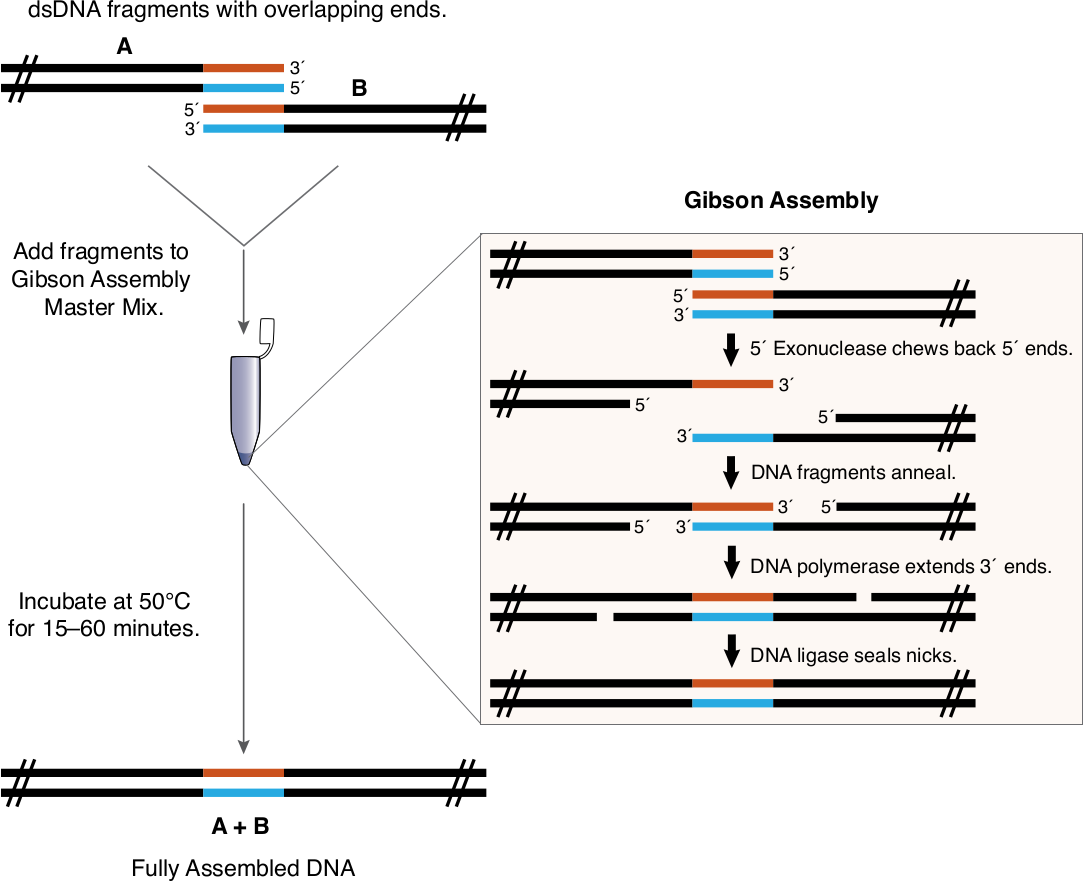
\includegraphics[width=0.8\textwidth, resolution=600, keepaspectratio=true]{graphics/gibson.png}}
			\caption[Overview of the Gibson assembly method]{Overview of the Gibson assembly method. Picture reproduced from the NEB Gibsson assembly master mix instruction manual NEB \#E2611S/L}
			\label{fig:gibson}
			\end{figure}				
		
		Once fragments of the desired size were obtained, the three PCR products were purified using the GE Healthcare Life Sciences Illustra-GRX PCR DNA and gel band purification kit and the concentration of DNA in the solution was estimated using the Nanodrop instrument. Simultaneously suicide plasmid vector pKAE604 was digested using Hind III and Sal I restriction enzymes. The digested product was purified and the concentration of the plasmid DNA was measured. For Gibson assembly NEB recommends a total DNA concentration of 0.2 to 1.0 pM when 4 to 6 DNA fragments are to be assembled. Therefore, for 4 fragments 0.25 pM is required and the weight in ng for each of the four fragments can be calculated with equation \ref{eq:gibson}. This allowed the volume required in $ \mu $l of the extracted DNA solutions to be determined. NEB recommends incubation of the Gibson Assembly master mix for an hour at 50\textcelsius.
		
		\begin{equation}
		\label{eq:gibson}
			weight \ in \ ng = \frac{pmols \times base \ pairs \times 650 \ daltons}{1000}
		\end{equation}
		
		\subsection{Transformation and validation}
		\label{sec:transformation}
		Following the Gibson assembly the ligated product was transformed into freshly prepared \textit{E. coli} DH5$ \alpha $ competent cells. As recommended by the NEB Gibson assembly protocol, the ligated product was diluted 4 fold (5 $ \mu $l of ligation in 15 $ \mu $l of deionised distilled water) prior to transformation. For transformation 2  $ \mu $l of the diluted product was added to 100  $ \mu $l of the competent cells and was held on ice for an hour. After an hour the cells were heat shocked for 90 sec at 42\textcelsius \ and then briefly returned to ice. The culture held on ice was mixed with 500  $ \mu $l of L-broth and was incubated at 37\textcelsius \ for an hour. Finally 200  $ \mu $l and 400  $ \mu $l of the culture was plated on to L-agar plates with kanamycin and grown at 37\textcelsius \ overnight.
		
		PCR was performed on the colonies picked from the transformation plates, using the left arm forward primer and the right arm reverse primer. The method for PCR was same as mentioned in the section \ref{sec:pcr} using the Taq polymerase enzyme. Table \ref{tab:validategibson} shows the PCR programme used for validating the ligation of the four fragments using Gibson assembly. The PCR product were analysed by 1 \% agarose gel electrophoresis. 

		\begin{table}[htbp]
		\caption{The PCR programme used for validating the product of Gibson assembly with the Taq DNA polymerase kit.}
		\label{tab:validategibson}
		\begin{center}
		\begin{tabular}{lrrr}
			\toprule[2pt]
			\textbf{Steps}          & \multicolumn{1}{l}{\textbf{Temperature (\textcelsius)}} & \multicolumn{1}{l}{\textbf{Time (sec)}} & \multicolumn{1}{l}{\textbf{Cycle}} \\ \midrule[1pt]
			Initial denaturation    &                                                      94 &                                      180 &                                  1 \\
			Denaturation            &                                                      94 &                                      30 &                                 30 \\
			Annealing and extension &                                                      72 &                                      90 &                                 30 \\
			Long extension          &                                                      72 &                                     600 &                                  1 \\ \bottomrule[2pt]
		\end{tabular}
		\end{center}
		\end{table}
		
		Successful PCR products were purified and sequenced using primers designed previously by Dr. Joanne Hothersall. Those primers bind on the region outside the multiple cloning site in the pAKE604 plasmid. The validated sample(s) was used to transform freshly prepared \textit{E. coli} S17-1 competent cells and were grown on L-agar plates with kanamycin selection and a sample of the successful transformant was stored in the -80\textcelsius \ freezer. 
		
		\subsection{Conjugal transfer of the suicide vector into \textit{P. fluorescens}}
		\label{sec:mating}
		For mating, overnight cultures were prepared for the transformed \textit{E. coli} S17-1 and the two \textit{P. fluorescens} host strains. 1 ml of each of the two \textit{P. fluorescens} host strains was mixed separately with 1 ml of the transformed \textit{E. coli} S17-1 strain. 1 ml of the culture mixture was filtered through a millipore nylon filter using a syringe and the filters were placed face up on to an L-agar plate without any antibiotic and grown overnight at 30\textcelsius. The bacteria were washed off the filters with 1 ml of saline. 10$ ^{-5} $ fold serial dilutions were made using 100 $\mu$l of the cells washed in saline followed by plating 100 $\mu$l of each dilution onto minimal medium plates with kanamycin selection. The plates were grown at 30\textcelsius \ for three to four days till the colonies were visible and big enough to be picked easily.
		
		To detect the successful transfer of the plasmid into the \textit{P. fluorescens} $ \Delta $ACP4 and $ \Delta $MupH cells, colonies were subjected to PCR (as described in Table \ref{tab:validategibson}) with ACP-K24a specific primers using Taq DNA polymerase.  The PCR products were analysed using 1\% agarose gel.
			 
		\subsection{Sucrose selection and excisant validation}
		\label{sec:suc selection}
		After mating, the \textit{P. fluorescens} \textit{trans} conjugants were subject to sucrose selection. For the \textit{P. fluorescens} $ \Delta $ACP4 trans-conjugants, colonies were grown overnight in L-broth without any selection. For each of the overnight cultures, five serial dilutions of 10$ ^{-1} $ were made for a final dilution of 10$ ^{-5}$  and 100 $\mu$l of culture from each of the five dilution tubes was plated on L-agar plates with sucrose selection. The cells were grown at 30\textcelsius \ for 24 hrs. To confirm that the plasmid had successfully excised out of the \textit{P. fluorescens} strains, colonies were patched onto two plates carrying ampicillin and kanamycin respectively. The colonies which grew on the ampicillin plates but not on the kanamycin plates were the ones which had successfully excised the plasmid. Successful excisions were subjected to PCR (as described in Table \ref{tab:validategibson}) with ACP-K24a specific primers using Taq DNA polymerase, in order to detect the integration of the ACP-K24a into \textit{P. fluorescens} $ \Delta $ACP4 chromosome.

		The previous steps validated the integration of the ACP-K24a into the \textit{P. fluorescens} $ \Delta $ACP4 chromosome but did not detect whether the integration had happened at the correct position in the \textit{mup} cluster. To validate that ACP-K24a had integrated at the correct position another PCR using Taq DNA polymerase was carried out. Primers designed previously by Dr. Anthony Haines, which bind to the positions outside the left and right arms were used with the annealing temperature of 53\textcelsius \ (as described in Table \ref{tab:validategibson}, with separate annealing and extension steps). \textit{P. fluorescens} NCIMB 10586 and \textit{P. fluorescens} $ \Delta $ACP4 were used as the controls. The PCR products were further subjected to restriction digests using enzymes Blp I and Stu I. Blp I cuts in the middle of the ACP-K24a but not does not cut anywhere in ACP-mupA3a and Stu I cuts in the middle of the ACP-mupA3a as well as at the rear ends of the two arms. A 20$\mu$l restriction digestion reaction mixture consists of DNA (5$\mu$l), Buffer (2$\mu$l), BSA (1$\mu$l), enzyme (conc. 5 units/$\mu$l) and enough sterile distilled water to make the total volume of 20$\mu$l. The restriction digest fragments were analysed by electrophoresis on 1\% agarose gel, an uncut fragment was used as the control. 
		
		For \textit{P. fluorescens} $ \Delta $MupH trans-conjugants sucrose selection was performed following the same steps as that for the \textit{P. fluorescens} $ \Delta $ACP4 trans-conjugants. However, to validate the excisions and integrants, samples were subjected to PCR using the primers designed to bind to the region outside the two arms. The steps of PCR with ACP-K24a specific primers and subsequent restriction digestions were excluded, since running a PCR using only the outer primers and sequencing the PCR products gave the same result in fewer steps and less time as compared to the above mentioned steps. 

		\subsection{Overlay Bioassay for \textit{in trans} expression of MupH, BatC and BatC L218M mutant}
		\label{sec:bioassay}
	
		For the bioassay 20 ml measured L-agar plates were made. The \textit{P. fluorescens} $ \Delta $H-6d strain carrying one of MupH, BatC or Batc L218M \textit{in trans} and the $ \Delta $4-1a  strain carrying the BatC \textit{in trans} were grown overnight in 5 ml L-broth with ampicillin selection. \textit{P. fluorescens} NCIMB 10586, $\Delta $MupH,  $ \Delta $ACP4, $ \Delta $H-6d and $ \Delta $4-1a were also grown without any plasmids, as controls. 100 $\mu$l of the overnight cultures were diluted with 900 $\mu$l of L-broth. To keep the concentration of the cells the same in all the cultures, the optical density of the samples was measured at 600 nm. Using equation \ref{eq:ODbioassay}, further dilutions were made keeping the total volume of the sample as 1 ml. 
		
		\begin{equation}
		\label{eq:ODbioassay}
		volume \ of \ the \ sample \ to \ dilute = \frac{smallest \ OD_{600}}{individual \ sample  \ OD_{600}} \times 1000
		\end{equation} 
		
		10 $ \mu $l of the diluted samples were spotted onto the 20 ml L-agar plates and were grown for 24 hr on the bench at room temperature. Simultaneously an overnight culture of \textit{Bacillus subtilis} 1064 strain was grown at 37\textcelsius. To prepare the overlay medium 4 ml of \textit{Bacillus subtilis} culture were mixed in 100 ml of molten L-agar and 500 $ \mu $l of TTC (5\% w/v). 15 ml of the overlay medium were poured over the spots from the 24 hr grown \textit{P. fluorescens} strains and were allowed to settle till the agar solidified, followed by a 24 hr incubation at 30\textcelsius. The diameters of the clearance zones were measured in two different directions, subtracting the diameter of the central disk. 
		  
		\subsection{High performance liquid chromatography analysis}
		\label{sec:hplc}
		To order to detect the pseudomonic acids produced by the \textit{in trans} expression of \textit{mupH}, \textit{batC} and \textit{batC} L218M in the ACP-K24a mutant \textit{P. fluorescens} strains, high performance liquid chromatography (HPLC) \nomenclature{HPLC}{High performance liquid chromatography} was performed. \textit{P. fluorescens} NCIMB 10586 and \textit{P. fluorescens} $ \Delta $H-6d and $ \Delta $4-1a with an empty pJH10 plasmid were used as controls. The seed cultures were prepared by growing the strains for 16 hr in L-broth at 25\textcelsius, 200 rpm. From the seed cultures, 1.25 ml of each sample was inoculated into  25 ml of the secondary stage medium (SSM). The inoculated cultures were grown at 22\textcelsius, 200 rpm for 40 hr. The cultures were pelleted in Falcon tubes by centrifugation at 5000 X g, at 25\textcelsius \ for 40 min. The supernatant was separated and filtered using 0.2 $ \mu $m Acrodiscs Nylon filters (Pall-Gelman, labs) before injection into the HPLC machine.
		
		The HPLC machine (Gilson) was supplied with HPLC grade water (Fisher) and 100\% aceto nitrile (Fisher) as mobile phase. The two solvents were added with 0.01\% formic acid (v/v) for pH adjustment and were degassed using an aspirator to remove any dissolved air prior to injection into the machine. The machine was set at 0.002 AUFS  (absorbance units full scale) \nomenclature{AUFS}{Absorbance units full scale} sensitivity and the detection was carried out at the wavelength of 233 nm. A Supelco reverse phase C18 column (15cm X 4.6 mm, 5$ \mu $m), which had hydrophobic alkyl chains covalently attached to the silica beads, was used to bind the hydrophobic compounds. Elution was performed by using a 5-70\% acetonitrile-water gradient at 1ml/min flow rate for 1 hr. Unipoint software was used to run the programme and analyse the chromatograms. 
		
		
		
		
		
		
		
		
		
		
		
		
		